\documentclass[spanish]{beamer}
\usepackage[T1]{fontenc}
\usepackage[utf8]{inputenc}
\usepackage{babel}
\usepackage{lmodern}
\usepackage{tikz}
\usepackage[vlined]{algorithm2e}
\usepackage{xcolor}
\usepackage{graphicx}
\usepackage{tikz}
\usetikzlibrary{arrows,automata,positioning}
\usepackage{amsmath,amssymb,amsfonts}
\usepackage{dashrule}

\addto\shorthandsspanish{\spanishdeactivate{~<>}}

\makeatletter
 \newcommand\makebeamertitle{\frame{\maketitle}}%
 % (ERT) argument for the TOC
 \AtBeginDocument{%
   \let\origtableofcontents=\tableofcontents
   \def\tableofcontents{\@ifnextchar[{\origtableofcontents}{\gobbletableofcontents}}
   \def\gobbletableofcontents#1{\origtableofcontents}
 }
\makeatother

\usetheme{Frankfurt}
\usecolortheme{crane}
\setbeamercovered{transparent}
\usefonttheme[onlymath]{serif}

%----Símbolos matemáticos definidos por ISO 80000-2:2009------------------------
\newcommand{\defeq}{\mathrel{\mathop:}=} %El signo de "igual por definición"
\let\gets\defeq
\newcommand{\transpose}[1]{{#1}^{\operatorname{T}}} %Operadores en letra derecha
\newcommand{\invert}[1]{{#1}^{-1}}
\newcommand{\bigOh}[1]{\operatorname{O}\left( #1 \right)}

\newcommand{\dist}[2]{\mathit{d}\left(#1 , #2\right)} %Excepto la distancia

\newcommand{\mat}[1]{\boldsymbol{#1}} %Las matrices van en negrita itálica
\renewcommand{\vec}[1]{\boldsymbol{#1}} %...y los vectores también
\newcommand{\entry}[3]{\left({#1}\right)_{{#2}\,{#3}}} %Entrada de una matriz
\newcommand{\sgn}{\operatorname{sgn}}
\newcommand{\abs}[1]{\left|{#1}\right|}

\newcommand{\Set}[1]{\left\{{#1}\right\}}
\newcommand{\Tuple}[1]{\left({#1}\right)}
\newcommand{\BuildSet}[2]{\left\{ #1 \middle| #2 \right\}}
\newcommand{\Nset}{\ensuremath{\mathbf{N}}} %Conjuntos numéricos en negrita
\newcommand{\Zset}{\ensuremath{\mathbf{Z}}}
\newcommand{\Rset}{\ensuremath{\mathbf{R}}}
\newcommand{\Cset}{\ensuremath{\mathbf{C}}}
\newcommand{\ident}{\ensuremath{\mat I}} %La matriz identidad se denota con I

\renewcommand{\leq}{\leqslant} %El símbolo menor-igual va inclinado
\renewcommand{\geq}{\geqslant} %...y también el mayor-igual
\let\le\leq
\let\ge\geq

%----Símbolos propios de este documento-----------------------------------------
\newcommand{\DynA}{\ensuremath{\mathbb{A}}} %Tipos Dynkin
\newcommand{\DynAtilde}{\ensuremath{\tilde{\mathbb{A}}}}
\newcommand{\DynB}{\ensuremath{\mathbb{B}}}
\newcommand{\DynC}{\ensuremath{\mathbb{C}}}
\newcommand{\DynD}{\ensuremath{\mathbb{D}}}
\newcommand{\DynDtilde}{\ensuremath{\tilde{\mathbb{D}}}}
\newcommand{\DynE}{\ensuremath{\mathbb{E}}}
\newcommand{\DynEtilde}{\ensuremath{\mathbb{E}}}
\newcommand{\DynF}{\ensuremath{\mathbb{F}}}
\newcommand{\DynG}{\ensuremath{\mathbb{G}}}
\newcommand{\intmatrix}[2]{\Zset^{#1\times #2}}
\newcommand{\diagmatrix}[1]{\mathrm{diag}\left(#1\right)}

\newcommand{\MultSymbol}{\epsilon}
\newcommand{\Mult}[2][]{\MultiplicitySymbol_{#1}\left({#2}\right)}

\newcommand{\MatrixSet}[2][n \times n]{\mathcal{M}_{#1}\left(#2\right)}
\newcommand{\qCclass}{\mathbf{qC}}
\newcommand{\sqCclass}{\mathbf{sqC}}
\newcommand{\Quadratic}[1]{\mathbf{q}_{#1}}
\newcommand{\Elementary}[3]{\ensuremath{\mat{E}_{{#1} \, {#2}}^{#3}}}
\newcommand{\Flation}[3]{\ensuremath{\FlationOp{{#1}}{{#2}}\left({#3}\right)}}
\newcommand{\FlationOp}[2]{\ensuremath{T_{{#1}\,{#2}}}}
\newcommand{\Roots}[1]{\mathcal{R}\left({#1}\right)}
\newcommand{\PositiveRoots}[1]{\mathcal{R}^{+}\left({#1}\right)}
\newcommand{\MatEdge}[2]{\mat{F}^{\left({#1},{#2}\right)}}

%Teoría de grafos
\newcommand{\Grafo}[2]{\mathbf{Grafo}\left({#1},{#2}\right)}
\tikzset{%
  every node/.style={circle, draw, inner sep = 1pt, fill = white},
  every path/.style={line width = 0.7pt, >=latex}%, line cap = round}
}

\pgfdeclarelayer{bg}    % declare background layer
\pgfsetlayers{bg,main}  % set the order of the layers (main is the standard)

\newcommand{\frontier}[2][]{\delta_{#1}\left({#2}\right)}
\newcommand{\VertexSet}[1]{\mathit{V}\left({#1}\right)}
\newcommand{\EdgeSet}[1]{\mathit{E}\left({#1}\right)}
\newcommand{\Adj}[1]{\operatorname{\mathbf{Adj}}\left({#1}\right)}
\newcommand{\Neighbours}[1]{N\left({#1}\right)}
\newcommand{\arista}[2]{\ensuremath{{#1}\EUS{#2}}}
\newcommand{\arco}[2]{\ensuremath{\left(#1,#2\right)}}
\newcommand{\BT}[1]{\mathrm{BT}\left(#1\right)} %Árbol de bloques
\newcommand{\blockset}{\mathcal{B}}
\newcommand{\grad}[2][]{d_{#1}\left(#2\right)}

%Algoritmos en grafos
\newcommand{\pre}[1]{\mathit{pre}\left[{#1}\right]}
\newcommand{\pos}[1]{\mathit{pos}\left[{#1}\right]}
\newcommand{\lowpoint}[1]{\mathit{sup}\left[{#1}\right]}
\newcommand{\padre}[1]{\mathit{padre}\left[{#1}\right]}
\newcommand{\List}[1]{\left[{#1}\right]}

%Teoría de bigrafos
\newcommand{\Bigraph}[1]{\mathbf{bigr}\left({#1}\right)}
\newcommand{\Biadj}[1]{\mathbf{biadj}\left({#1}\right)}
\newcommand{\Simp}[1]{\operatorname{\mathbf{simp}}\left({#1}\right)}
\newcommand{\Marco}[1]{\Phi\left({#1}\right)}
\newcommand{\Oset}{\mathcal{O}}
\newcommand{\Full}[2]{\mathbf{F}\left[{#1}, {#2}\right]}
\newcommand{\Fclass}{\mathcal{F}}
\newcommand{\solida}{\ensuremath{\mathtt{sólida}}}

% inline undirected dotted edge
\newcommand{\EUD}{
  \begin{tikzpicture}[baseline = -0.5ex]
  \draw[dotted] (0, 0) -- (0.5, 0);
  \end{tikzpicture}  
}

% Undirected solid edge
\newcommand{\EUS}{
  \begin{tikzpicture}[baseline = -0.5ex]
  \draw (0, 0) -- (0.5, 0);
  \end{tikzpicture}  
}

% Undirected solid edge
\newcommand{\EUU}{
  
\begin{tikzpicture}[baseline = -0.5ex]
  \draw[line width = 2, color = gray] (0, 0) -- (0.5, 0);
  \end{tikzpicture}  
}

% Directed solid edge
\newcommand{\EDS}{
  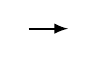
\begin{tikzpicture}[baseline = -0.5ex]
  \draw[->] (0, 0) -- (0.5, 0);
  \end{tikzpicture}  
}

% Directed dotted edge
\newcommand{\EDD}{
  \begin{tikzpicture}[baseline = -0.5ex]
  \draw[->, dotted] (0, 0) -- (0.5, 0);
  \end{tikzpicture}
}

%Análisis léxico
\newcommand{\str}[1]{\textbf{\texttt{#1}}}
\newcommand{\dash}{\text{--}}

%Recuadros
\definecolor{FondoRecuadro}{rgb}{0.90,0.90,1.0}
\makeatletter
\newenvironment{recuadro}{%
  \noindent%
  \begin{lrbox}{\@tempboxa}\begin{minipage}{\columnwidth}}{\end{minipage}\end{lrbox}%
  \colorbox{FondoRecuadro}{\usebox{\@tempboxa}}
}
\makeatother

%----Pseudocódigo---------------------------------------------------------------
\SetKwProg{Function}{función}{:}{}
\SetKwIF{If}{ElseIf}{Else}{si}{:}{en otro caso, si}{en otro caso:}{}
\SetKwFor{For}{para}{:}{}
\SetKwFor{While}{repetir mientras}{:}{}
\SetKwRepeat{Repeat}{repetir:}{hasta que}{}
\SetKwFor{ForEach}{para cada}{:}{}
\SetKw{KwFrom}{desde}
\SetKw{KwTo}{hasta}
\SetKw{Return}{devolver}
\SetKw{New}{nuevo}
\SetKw{KwAnd}{y}
\SetKw{KwAndE}{e}
\SetKw{KwOr}{o}
\SetKw{KwNot}{no}
\SetKw{Print}{imprimir}
\SetKwComment{tcp}{$\blacktriangleright$}{}
\SetKwInput{KwIn}{entrada}
\SetKwInput{KwOut}{salida}
\newcommand{\None}{\textsc{Ninguno}}
\newcommand{\False}{\textsc{Falso}}
\newcommand{\True}{\textsc{Verdadero}}

\begin{document}
\title[Clasificación Dynkin]{Clasificación algorítmica en gráficas de tipo
$\mathbb{D}_n$}

\author[R. Gutiérrez]{Rey David Gutiérrez Torres\\ Daniel Rivera López}

\institute[UAEM]{Universidad Autónoma del Estado de Morelos}

%\date{21 de junio de 2017}

\makebeamertitle

\pgfdeclareimage[height=0.5cm]{institution-logo}{logoUAEM}
\logo{\pgfuseimage{institution-logo}}

\AtBeginSubsection[]{%
  \frame<beamer>{ 
    \frametitle{Índice}   
    \tableofcontents[currentsection, currentsubsection] 
  }
}

%\beamerdefaultoverlayspecification{<+->}

\begin{frame}{Índice}
  \tableofcontents{}
\end{frame}

\section{Conceptos y relaciones}

\begin{frame}{Matriz de Cartan simétrica}
  \begin{columns}
    \begin{column}{5cm}
        \begin{definition}
          \begin{itemize}
            \item<+->  Una matriz $\mat{A} \in \MatrixSet{\mathbb{Z}}$ es 
            \textbf{casi Cartan simétrica} si $\mat{A}$ es simétrica y $\entry{\mat{A}}{i}{i} = 2$ para toda $i = 1, \ldots, n$.
            \item<+-> Se denotan por $\sqCclass$.
          \end{itemize}      
        \end{definition}
    \end{column}
    \begin{column}{5cm}
      \begin{example}<+->
        \begin{equation*}
        \begin{pmatrix}
        2 & -2 & 1 & 0\\
        -2 & 2 & -1 & 0\\
        1 & -1 & 2 & 1\\
        0 & 0 & 1 & 2\\
        \end{pmatrix}
        \end{equation*}
      \end{example}
    \end{column}
  \end{columns}
\end{frame}

\begin{frame}{Forma cuadrática}
  \framesubtitle{}{}
  \begin{itemize}
  \item Una forma cuadrática es un polinomio $q : \mathbb{R}^{n} \rightarrow \mathbb{R}$ con $n > 0$ si cada monomio del mismo es una variable al cuadrado o la multiplicación de dos variables. Esto es equivalente a decir que $q$ se puede expresar como:
	\begin{align*}
    q\left(x_1, x_2,\ldots, x_n\right) &=  \sum_{i=1}^{n}q_{ii}\,x_{i}^{2} + \sum_{1 \leq i \leq j \leq n}q_{ij\,}x_{i}\,x_{j}
  \end{align*}
  \item Una forma cuadrática unitaria es un caso especial donde $q_{ii}=1$
  \end{itemize}
\end{frame}

\begin{frame}{Forma unitaria asociada a una matriz casi Cartan}
  \framesubtitle{Matriz casi-Cartan simétrica $\leftrightarrow$ Forma unitaria}
  \begin{align*}
    \Quadratic{\mat{A}}\left(\vec{x}\right) &= \frac{1}{2} 
    \transpose{\vec{x}} \mat{A} \vec{x}  \pause \\
    &= \frac{1}{2} \left( \sum_{i = 1}^{n} \sum_{j = 1}^{n} 
      \entry{\mat{A}}{i}{j} x_i x_j \right) \pause \\
    &= \frac{1}{2} \left(\sum_{i=1}^{n} \entry{\mat{A}}{i}{i} x_i^2
       + 2 \sum_{1 \le i < j \le n} \entry{\mat{A}}{i}{j} x_i x_j\right)  
       \pause \\
    &= \sum_{i=1}^{n} x_i^2 + \sum_{1 \le i < j \le n} \entry{\mat{A}}{i}{j}    
       x_i x_j \text{.}
  \end{align*}
\end{frame}

\begin{frame}{Forma unitaria asociada a una matriz casi Cartan}
  \begin{definition}
  Una matriz casi Cartan simétrica $A$ es \textbf{definida positiva} si y sólo si 
  $\Quadratic{\mat{A}}\left(\vec{x}\right) = \frac{1}{2} \transpose{\vec{x}} \mat{A} \vec{x}>0$, para toda $x\in \mathbb{Z}$ con $x\neq \vec{0}$.
  \end{definition}
\end{frame}


\begin{frame}{Bigráfica asociada a una matriz casi Cartan}
  \framesubtitle{Matriz casi-Cartan simétrica $\leftrightarrow$ Bigráfica}
  \begin{theorem}
    Sea $A\in M_{n}(\mathbb{Z})$ una matriz casi Cartan simétrica y definida positiva sean  $i,j\in\{1,2...n\}$, entonces, 
\begin{enumerate}
\item [$(a)$] $0\leq A_{ij}A_{ji}<4$ 
\item [$(b)$] $A_{ij}\in\{-1,0,1\}$\end{enumerate}  \end{theorem}\pause
La bigráfica $\Bigraph{\mat{A}}$ asociada a la matriz $A$  tiene  vértices $\left\{ 1,2,\ldots,n\right\} $, y para cada par de vértices $i$, $j$ con $i\neq j$:\pause
	\begin{enumerate}
		\item Si $A_{ij}=-1=A_{ji}$ trazamos una arista solida entre los vértices,
		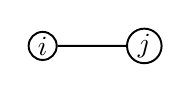
\begin{tikzpicture}[baseline = (v1.base), scale = 1.5]
      \node (v1) at (-0.8604975358129109, -0.4070708333164735) {$i$};   
      \node (v2) at (0.000, -0.4070708333164735) {$j$};
      \draw (v1)--(v2);  
       \end{tikzpicture}\pause
		\item Si $A_{ij}=1=A_{ji}$ trazamos una arista punteada entre los vértices, 
		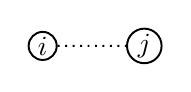
\begin{tikzpicture}[baseline = (v1.base), scale = 1.5]
      \node (v1) at (-0.8604975358129109, -0.4070708333164735) {$i$};   
      \node (v2) at (0.000, -0.4070708333164735) {$j$};
      \draw[dotted] (v1)--(v2);  
       \end{tikzpicture}
	\end{enumerate}
 \end{frame}

\begin{frame}{Equivalencia de conceptos}
  \framesubtitle{Ejemplo}
  $\mat{A} =
  \begin{pmatrix}
    2 & -1 & 0 & 1\\
    -1 & 2 & 1 & 1\\
    0 & 1 & 2 & 0\\
    1 & 1 & 0 & 2\\
  \end{pmatrix}$\pause
  \qquad
  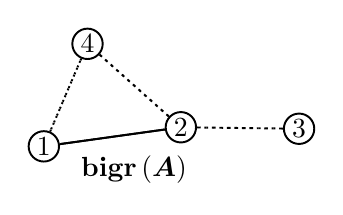
\begin{tikzpicture}[baseline = (v3.base), scale = 0.9]
  \node (v0) at (-0.7604975358129109, -0.9070708333164735) {$1$};
  \node (v1) at (1.1732333853473758, -0.63758645858272716) {$2$};
  \node (v2) at (2.84142321122027776, -0.6585990909663623) {$3$};
  \node (v3) at (-0.144076010236877, 0.5397895385876869) {$4$};
  \begin{pgfonlayer}{bg}
  \draw (v0) -- (v1);
  \draw[dotted] (v0) -- (v3);
  \draw (v1) -- (v0);
  \draw[dotted] (v1) -- (v2);
  \draw[dotted] (v1) -- (v3);
  \draw[dotted] (v2) -- (v1);
  \draw[dotted] (v3) -- (v0);
  \draw[dotted] (v3) -- (v1);
  \end{pgfonlayer}
  \node[draw = none, shape = rectangle] (t) at (0.51273585,-1.237586459) 
  {$\Bigraph{\mat{A}}$};
  \end{tikzpicture}\pause
  \begin{equation*}
    \Quadratic{\mat{A}}\left(x_1, x_2, x_3, x_4\right) = x_1^2 + x_2^2 + x_3^2 
    + x_4^2 - x_1 x_2 + x_1 x_4 + x_2 x_3 + x_2 x_4
  \end{equation*}
\end{frame}

\begin{frame}{$\Zset$-equivalencia}
  \begin{definitions}
    \begin{itemize}
      \item<+-> Una matriz $\mat{M} \in \MatrixSet{\Zset}$ es 
        \Zset-invertible si tiene inversa $\mat{M}^{-1} \in 
        \MatrixSet{\Zset}$.
      \item<+-> $\mat{A}, \mat{A^{\prime}} \in \sqCclass$ son 
      \Zset-equivalentes si existe una matriz $\Zset$-invertible 
      $\mat{M}$ tal que $\mat{A}^\prime = \transpose{\mat{M}} \mat{A} \mat{M}$.
    \end{itemize}
  \end{definitions}
\end{frame}

\begin{frame}{Diagramas de Dynkin}
  \begin{itemize}
    \item Todas las bigráficas conexas, definidas positivas, de aristas sólidas:
  \end{itemize}
  \pause
  \begin{tabular}{ll}
    Familia & Gráfica\\
    $\DynA_{n}$, $n\ge1$ &
    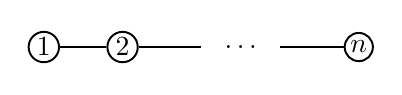
\begin{tikzpicture}
    [baseline=(v1.base)]
    \node (v1) at (0, 0) {$1$};
    \node (v2) at (1, 0) {$2$};
    \node (v3) at (4, 0) {$n$};
    \node[draw = none] (v5) at (2.5, 0) {$\ldots$};
    \draw (v1) -- (v2) -- (2, 0);
    \draw (3, 0) -- (v3);
    \end{tikzpicture} \pause \\
    $\DynD_{n}$, $n\ge4$ &
    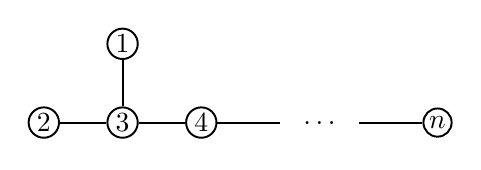
\begin{tikzpicture}
    [baseline=(v1.base)]
    \node (v1) at (0, 0) {$2$};
    \node (v2) at (1, 0) {$3$};
    \node (v3) at (2, 0) {$4$};
    \node (v4) at (5, 0) {$n$};
    \node (v5) at (1, 1) {$1$};
    \node[draw = none] (dots) at (3.5, 0) {$\ldots$};
    \draw (v1) -- (v2) -- (v3) -- (3, 0); \draw (v5)
    -- (v2); \draw (4, 0) -- (v4);
    \end{tikzpicture}\pause \\
    $\DynE_{n}$, $6\le n\le8$ &
    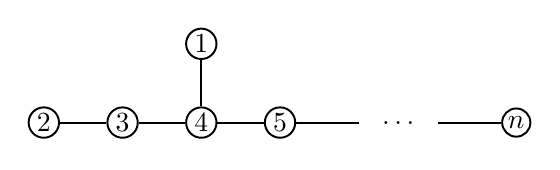
\begin{tikzpicture} [baseline=(v1.base)]
    \node (v1) at (0, 0) {$2$};
    \node (v2) at (1, 0) {$3$};
    \node (v3) at (2, 0) {$4$};
    \node (v4) at (3, 0) {$5$};
    \node (v5) at (6, 0) {$n$};
    \node (v6) at (2, 1) {$1$};
    \node[draw = none] (dots) at (4.5, 0) {$\ldots$};
    \draw (v1) -- (v2) -- (v3) -- (v4) -- (4, 0);
    \draw (v6) -- (v3);
    \draw (5, 0) -- (v5);
    \end{tikzpicture}\\
  \end{tabular}
\end{frame}

\begin{frame}{La clasificación $\DynA-\DynD-\DynE$}
  \begin{theorem}<+->[S. Ovsienko -- 1978]
    Toda bigráfica $G$ conexa y definida positiva es \Zset-equivalente a un diagrama de Dynkin.
  \end{theorem}
  \begin{proof}
   Demostración constructiva mediante el \textbf{algoritmo de las inflaciones}.
  \end{proof}
\end{frame}

\section{Algoritmo de las inflaciones}
\begin{frame}{Inflaciones}
  \begin{definitions}
    \begin{itemize}[<+->]
      \item $\mat{I}$ denota la matriz identidad con vectores columna 
      $\vec{e}_j$.
      \item $\Elementary{s}{r}{\sigma} \defeq \mat{I} + \sigma \, \vec{e}_s \, 
      \transpose{\vec{e}_r}$ ($s, r \in \Set{1, \ldots, n}$, $\sigma \in 
      \mathbb{R}$) denota una \textbf{matriz elemental} de suma de renglones/columnas.
      \item Si $\mat{A} \in \sqCclass$ y $\entry{\mat{A}}{s}{r} = 1$ entonces 
      $\transpose{\left(\Elementary{s}{r}{-1}\right)} \mat{A} 
      \left(\Elementary{s}{r}{-1}\right)$ es una \textbf{inflación} de $\mat{A}$.
    \end{itemize}
  \end{definitions}
\end{frame}

\begin{frame}{Algoritmo de las inflaciones}
  \begin{block}{Algoritmo de las inflaciones}<+->
  \SetKwFunction{Inflaciones}{inflaciones}
    \begin{algorithm}[H]
      \Function{\Inflaciones{$\mat{A}$}}{
        \While{exista una entrada no diagonal $\entry{\mat{A}}{s}{r} = 1$}{
          $\mat{A} \gets \transpose{\left(\Elementary{s}{r}{-1}\right)} \, 
          \mat{A} 
          \, \left(\Elementary{s}{r}{-1}\right)$
        }
      }
    \end{algorithm}
  \end{block}
\end{frame}

\begin{frame}[label=ejemploInflacion]{Interpretación gráfica}
  \begin{example}<1->[$\Flation{1}{5}{G}$]
    \centering
    \only{
      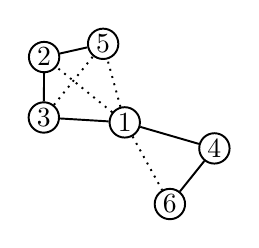
\begin{tikzpicture}
      \node (v1) at (0.5783140174240109, -0.3166613786083942) {$1$};
      \node (v2) at (-0.44575835363976835, 0.5128328399021246) {$2$};
      \node (v3) at (-0.44938111110291284, -0.2545625932461614) {$3$};
      \node (v4) at (1.7169249235942454, -0.6471916538729541) {$4$};
      \node (v5) at (0.3039359827412884, 0.6808427684519154) {$5$};
      \node (v6) at (1.1515342924415832, -1.353600447175456) {$6$};
      \draw[dotted] (v1) -- (v2);
      \draw (v1) -- (v3);
      \draw (v1) -- (v4);
      \draw[dotted] (v1) -- (v5);
      \draw[dotted] (v1) -- (v6);
      \draw (v2) -- (v3);
      \draw (v2) -- (v5);
      \draw[dotted] (v3) -- (v5);
      \draw (v4) -- (v6);
      \end{tikzpicture}
    }<1>
    \only{
      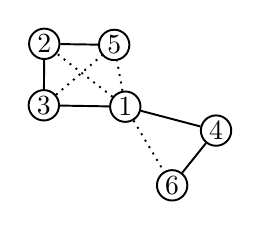
\begin{tikzpicture}
      \node (v1) at (0.5412198978114261, -0.30837975982599586) {$1$};
      \node (v2) at (-0.48785274767316644, 0.489844710272699) {$2$};
      \node (v3) at (-0.4933754862393873, -0.2907417156736922) {$3$};
      \node (v4) at (1.6939482240034156, -0.6120585870010133) {$4$};
      \node (v5) at (0.40000368649860146, 0.4762208321087451) {$5$};
      \node (v6) at (1.1362237482385447, -1.307276832397221) {$6$};
      \draw[dotted] (v1) -- (v2);
      \draw (v1) -- (v3);
      \draw (v1) -- (v4);
      \draw[dotted] (v1) -- (v5);
      \draw[dotted] (v1) -- (v6);
      \draw (v2) -- (v3);
      \draw (v2) -- (v5);
      \draw[dotted] (v3) -- (v5);
      \draw (v4) -- (v6);
      \end{tikzpicture}
    }<2>
    \only{
      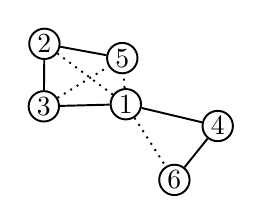
\begin{tikzpicture}
      \node (v1) at (0.5041257781988414, -0.30009814104359744) {$1$};
      \node (v2) at (-0.5299471417065647, 0.4668565806432734) {$2$};
      \node (v3) at (-0.5373698613758617, -0.3269208381012231) {$3$};
      \node (v4) at (1.670971524412586, -0.5769255201290725) {$4$};
      \node (v5) at (0.45906032004567493, 0.28561630232156) {$5$};
      \node (v6) at (1.120913204035506, -1.2609532176189864) {$6$};
      \draw[dotted] (v1) -- (v2);
      \draw (v1) -- (v3);
      \draw (v1) -- (v4);
      \draw[dotted] (v1) -- (v5);
      \draw[dotted] (v1) -- (v6);
      \draw (v2) -- (v3);
      \draw (v2) -- (v5);
      \draw[dotted] (v3) -- (v5);
      \draw (v4) -- (v6);
      \end{tikzpicture}
    }<3>
    \only{
      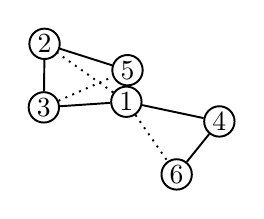
\begin{tikzpicture}
      \node (v1) at (0.4670316585862566, -0.2918165222611991) {$1$};
      \node (v2) at (-0.5720415357399629, 0.4438684510138479) {$2$};
      \node (v3) at (-0.5813642365123363, -0.36309996052875393) {$3$};
      \node (v4) at (1.647994824821756, -0.5417924532571318) {$4$};
      \node (v5) at (0.4811058833825087, 0.10902917909036036) {$5$};
      \node (v6) at (1.1056026598324675, -1.2146296028407517) {$6$};
      \draw[dotted] (v1) -- (v2);
      \draw (v1) -- (v3);
      \draw (v1) -- (v4);
      \draw[dotted] (v1) -- (v5);
      \draw[dotted] (v1) -- (v6);
      \draw (v2) -- (v3);
      \draw (v2) -- (v5);
      \draw[dotted] (v3) -- (v5);
      \draw (v4) -- (v6);
      \end{tikzpicture}
    }<4>
    \only{
      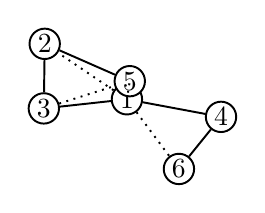
\begin{tikzpicture}
      \node (v1) at (0.4299375389736718, -0.2835349034788007) {$1$};
      \node (v2) at (-0.6141359297733611, 0.42088032138442233) {$2$};
      \node (v3) at (-0.6253586116488108, -0.39927908295628484) {$3$};
      \node (v4) at (1.6250181252309264, -0.5066593863851909) {$4$};
      \node (v5) at (0.4661403765091028, -0.05354053758485405) {$5$};
      \node (v6) at (1.090292115629429, -1.168305988062517) {$6$};
      \draw[dotted] (v1) -- (v2);
      \draw (v1) -- (v3);
      \draw (v1) -- (v4);
      \draw[dotted] (v1) -- (v5);
      \draw[dotted] (v1) -- (v6);
      \draw (v2) -- (v3);
      \draw (v2) -- (v5);
      \draw[dotted] (v3) -- (v5);
      \draw (v4) -- (v6);
      \end{tikzpicture}
    }<5>
    \only{
      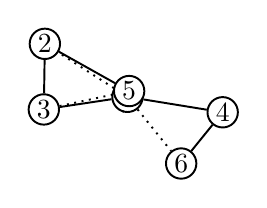
\begin{tikzpicture}
      \node (v1) at (0.3928434193610871, -0.27525328469640237) {$1$};
      \node (v2) at (-0.6562303238067592, 0.3978921917549967) {$2$};
      \node (v3) at (-0.6693529867852852, -0.43545820538381563) {$3$};
      \node (v4) at (1.6020414256400966, -0.4715263195132502) {$4$};
      \node (v5) at (0.41416379942545734, -0.20209284770408312) {$5$};
      \node (v6) at (1.0749815714263902, -1.1219823732842822) {$6$};
      \draw[dotted] (v1) -- (v2);
      \draw (v1) -- (v3);
      \draw (v1) -- (v4);
      \draw[dotted] (v1) -- (v5);
      \draw[dotted] (v1) -- (v6);
      \draw (v2) -- (v3);
      \draw (v2) -- (v5);
      \draw[dotted] (v3) -- (v5);
      \draw (v4) -- (v6);
      \end{tikzpicture}
    }<6>
    \only{
      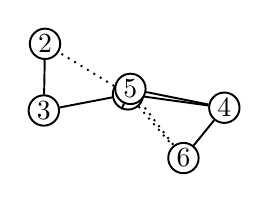
\begin{tikzpicture}
      \node (v1) at (0.35574929974850233, -0.266971665914004) {$1$};
      \node (v2) at (-0.6983247178401573, 0.37490406212557115) {$2$};
      \node (v3) at (-0.7133473619217596, -0.47163732781134654) {$3$};
      \node (v4) at (1.579064726049267, -0.4363932526413094) {$4$};
      \node (v5) at (0.3863224473654325, -0.19731558056068116) {$5$};
      \node (v6) at (1.0596710272233518, -1.0756587585060475) {$6$};
      \draw[dotted] (v1) -- (v2);
      \draw (v1) -- (v3);
      \draw (v1) -- (v4);
      \draw (v1) -- (v5);
      \draw[dotted] (v1) -- (v6);
      \draw (v2) -- (v3);
      \draw (v4) -- (v5);
      \draw (v4) -- (v6);
      \draw[dotted] (v5) -- (v6);
      \end{tikzpicture}
    }<7>
    \only{
      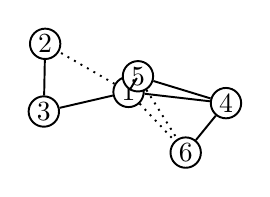
\begin{tikzpicture}
      \node (v1) at (0.31865518013591754, -0.2586900471316056) {$1$};
      \node (v2) at (-0.7404191118735555, 0.3519159324961456) {$2$};
      \node (v3) at (-0.7573417370582343, -0.5078164502388773) {$3$};
      \node (v4) at (1.5560880264584371, -0.4012601857693686) {$4$};
      \node (v5) at (0.4381329256443877, -0.060234845988625885) {$5$};
      \node (v6) at (1.044360483020313, -1.0293351437278129) {$6$};
      \draw[dotted] (v1) -- (v2);
      \draw (v1) -- (v3);
      \draw (v1) -- (v4);
      \draw (v1) -- (v5);
      \draw[dotted] (v1) -- (v6);
      \draw (v2) -- (v3);
      \draw (v4) -- (v5);
      \draw (v4) -- (v6);
      \draw[dotted] (v5) -- (v6);
      \end{tikzpicture}
    }<8>
    \only{
      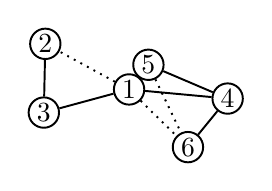
\begin{tikzpicture}
      \node (v1) at (0.2815610605233328, -0.25040842834920723) {$1$};
      \node (v2) at (-0.7825135059069537, 0.32892780286672) {$2$};
      \node (v3) at (-0.8013361121947087, -0.5439955726664083) {$3$};
      \node (v4) at (1.5331113268676075, -0.3661271188974279) {$4$};
      \node (v5) at (0.5269544741335828, 0.06282848202744401) {$5$};
      \node (v6) at (1.0290499388172745, -0.983011528949578) {$6$};
      \draw[dotted] (v1) -- (v2);
      \draw (v1) -- (v3);
      \draw (v1) -- (v4);
      \draw (v1) -- (v5);
      \draw[dotted] (v1) -- (v6);
      \draw (v2) -- (v3);
      \draw (v4) -- (v5);
      \draw (v4) -- (v6);
      \draw[dotted] (v5) -- (v6);
      \end{tikzpicture}
    }<9>
    \only{
      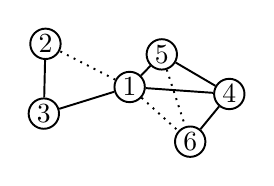
\begin{tikzpicture}
      \node (v1) at (0.24446694091074805, -0.24212680956680888) {$1$};
      \node (v2) at (-0.8246078999403518, 0.30593967323729443) {$2$};
      \node (v3) at (-0.8453304873311831, -0.5801746950939392) {$3$};
      \node (v4) at (1.5101346272767775, -0.33099405202548704) {$4$};
      \node (v5) at (0.6527870928330174, 0.17187440348752864) {$5$};
      \node (v6) at (1.013739394614236, -0.9366879141713432) {$6$};
      \draw[dotted] (v1) -- (v2);
      \draw (v1) -- (v3);
      \draw (v1) -- (v4);
      \draw (v1) -- (v5);
      \draw[dotted] (v1) -- (v6);
      \draw (v2) -- (v3);
      \draw (v4) -- (v5);
      \draw (v4) -- (v6);
      \draw[dotted] (v5) -- (v6);
      \end{tikzpicture}
    }<10>
    \only{
      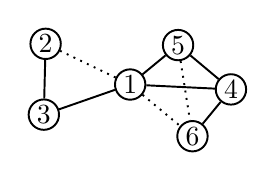
\begin{tikzpicture}
      \node (v1) at (0.2073728212981633, -0.23384519078441052) {$1$};
      \node (v2) at (-0.86670229397375, 0.2829515436078689) {$2$};
      \node (v3) at (-0.8893248624676576, -0.6163538175214699) {$3$};
      \node (v4) at (1.487157927685948, -0.2958609851535463) {$4$};
      \node (v5) at (0.8156307817426915, 0.2669029183916278) {$5$};
      \node (v6) at (0.9984288504111973, -0.8903642993931086) {$6$};
      \draw[dotted] (v1) -- (v2);
      \draw (v1) -- (v3);
      \draw (v1) -- (v4);
      \draw (v1) -- (v5);
      \draw[dotted] (v1) -- (v6);
      \draw (v2) -- (v3);
      \draw (v4) -- (v5);
      \draw (v4) -- (v6);
      \draw[dotted] (v5) -- (v6);
      \end{tikzpicture}
    }<11>
  \end{example}
\end{frame}

\section{Caso $\DynA_{n}$}

\begin{frame}{$\DynA$-bloques}
  \begin{definitions}
    \begin{itemize}[<+->]
      \item Sean $\mathrm{X}$ y $\mathrm{Y}$ conjuntos disjuntos de vértices. Denotamos por $\mathrm{F [X, Y]}$ el bigrafo no separable obtenido uniendo cada par de vértices $(x, y)$ con $x \in \mathrm{X}$ e $y \in \mathrm{Y}$ por una arista sólida, y todos los demás pares de vértices por una arista punteada, tal bigrafo se llama un $\DynA$ bloque.
    \end{itemize}
  \end{definitions}
  \begin{example}<+->
  \centering
  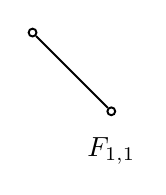
\begin{tikzpicture}[baseline=(current bounding box.center)]
  \node (v0) at (1, 0.0) {};
  \node (v1) at (0.0, 1) {};
  \draw (v0) -- (v1);
  \node[draw = none, shape = rectangle, fill=none] at (1, -0.5) {$F_{1,1}$};
  \end{tikzpicture}
  \qquad
  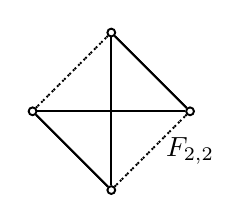
\begin{tikzpicture}[baseline=(current bounding box.center)]
  \node (v0) at (1, 0.0) {};
  \node (v1) at (-0.0, 1) {};
  \node (v2) at (-1, -0.0) {};
  \node (v3) at (0.0, -1) {};
  \draw (v0) -- (v1);
  \draw (v0) -- (v2);
  \draw[dotted] (v0) -- (v3);
  \draw (v1) -- (v0);
  \draw (v1) -- (v3);
  \draw[dotted] (v1) -- (v2);
  \draw (v2) -- (v3);
  \draw (v2) -- (v0);
  \draw[dotted] (v2) -- (v1);
  \draw (v3) -- (v1);
  \draw (v3) -- (v2);
  \draw[dotted] (v3) -- (v0);
  \node[draw = none, shape = rectangle, fill=none] at (1, -0.5) {$F_{2,2}$};
  \end{tikzpicture}
  \qquad
  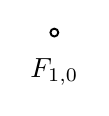
\begin{tikzpicture}[baseline=(current bounding box.center)]
  \node (v0) at (1, 0.0) {};
  \node[draw = none, shape = rectangle, fill=none] at (1, -0.5) {$F_{1,0}$};
  \end{tikzpicture}
  \qquad
  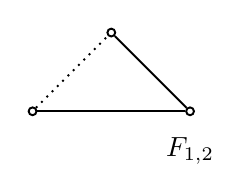
\begin{tikzpicture}[baseline=(current bounding box.center)]
  \node (v0) at (1, 0.0) {};
  \node (v1) at (-0.0, 1) {};
  \node (v2) at (-1, -0.0) {};
  \draw (v0) -- (v1);
  \draw (v0) -- (v2);
  \draw[dotted] (v2) -- (v1);
  \node[draw = none, shape = rectangle, fill=none] at (1, -0.5) {$F_{1,2}$};
  \end{tikzpicture}
  \end{example}
\end{frame}

\begin{frame}{Vértices de corte}
  \begin{definition}<+->[F. Harary -- 1969]
    Sea $G$ una gráfica.
    \begin{itemize}[<+->]
      \item $\kappa\left(G\right)$ denota a la cantidad de componentes conexas de $G$.
      \item $v \in \VertexSet{G}$ es un \textbf{vértice de corte} si  $\kappa\left(G\right) < \kappa\left(G - v\right)$.
    \end{itemize}
  \end{definition}
  \begin{example}<+->
    \centering
    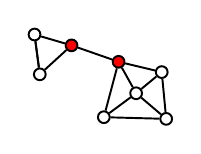
\begin{tikzpicture}[every node/.style={circle, draw, inner sep=1.5pt, fill=white}, 
      rotate=-45, scale=0.5]
  	\node[fill=red, text=white] (v0) at (-1.6, 0.45) {};
  	\node (v1) at (-1.65, -0.64) {};
  	\node (v2) at (-2.46, -0.02) {};
  	\node[fill=red, text=white] (v3) at (-0.46, 1.0) {};
  	\node (v4) at (0.5, 1.59) {};
  	\node (v5) at (1.42, 0.83) {};
  	\node (v6) at (0.27, -0.26) {};
  	\node (v7) at (0.42, 0.75) {};
  	\draw (v0) -- (v1);
  	\draw (v0) -- (v2);
  	\draw (v3) -- (v6);
  	\draw (v0) -- (v3);
  	\draw (v1) -- (v2);
  	\draw (v2) -- (v1);
  	\draw (v3) -- (v4);
  	\draw (v3) -- (v7);
  	\draw (v4) -- (v5);
  	\draw (v4) -- (v7);
  	\draw (v5) -- (v6);
  	\draw (v5) -- (v7);
  	\draw (v6) -- (v7);
	\end{tikzpicture}
  \end{example}
\end{frame}

\begin{frame}
\begin{lemma}
	Todo $\DynA$-bloque es de tipo $\DynA_{n}$
	\end{lemma}
	\begin{lemma}
	Sean $B_{1}$ y $B_{2}$ $\DynA$-bloques entonces $B_{1} + B_{2}$ es un $\DynA$-bloque
	\end{lemma}
  \begin{example}<1->[]
    \centering
      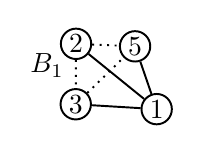
\begin{tikzpicture}[baseline=(current bounding box.center)]
      \node (v1) at (0.5783140174240109, -0.3166613786083942) {$1$};
      \node (v2) at (-0.44575835363976835, 0.5128328399021246) {$2$};
      \node (v3) at (-0.44938111110291284, -0.2545625932461614) {$3$};
      \node (v5) at (0.3039359827412884, 0.4808427684519154) {$5$};
      \draw (v1) -- (v2);
      \draw (v1) -- (v3);
      \draw (v1) -- (v5);
      \draw[dotted] (v2) -- (v3);
      \draw[dotted] (v2) -- (v5);
      \draw[dotted] (v3) -- (v5);
      \node[draw = none, shape = rectangle, fill=none] (t) at (-0.81273585,0.237586459) 
  {$B_1$};
      \end{tikzpicture}
      \quad
      \quad
     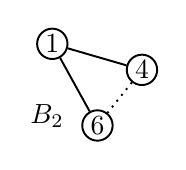
\begin{tikzpicture}[baseline=(current bounding box.center)]
     \node (v1) at (0.5783140174240109, -0.3166613786083942) {$1$};
      \node (v4) at (1.7169249235942454, -0.6471916538729541) {$4$};
      \node (v6) at (1.1515342924415832, -1.353600447175456) {$6$};
      \draw (v1) -- (v4);
      \draw (v1) -- (v6);
      \draw[dotted] (v4) -- (v6);
      \node[draw = none, shape = rectangle, fill=none] (t) at (0.51273585,-1.237586459) 
  {$B_2$};
      \end{tikzpicture}
  \end{example}
\end{frame}

\begin{frame}{$\DynA$-bloques}
  \begin{example}<1->[$\Flation{4}{6}{G}$]
    \centering
    \only{
      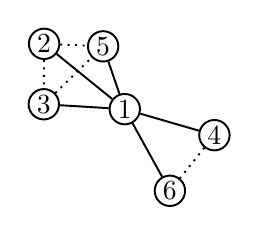
\begin{tikzpicture}
      \node (v1) at (0.5783140174240109, -0.3166613786083942) {$1$};
      \node (v2) at (-0.44575835363976835, 0.5128328399021246) {$2$};
      \node (v3) at (-0.44938111110291284, -0.2545625932461614) {$3$};
      \node (v4) at (1.7169249235942454, -0.6471916538729541) {$4$};
      \node (v5) at (0.3039359827412884, 0.4808427684519154) {$5$};
      \node (v6) at (1.1515342924415832, -1.353600447175456) {$6$};
      \draw (v1) -- (v2);
      \draw (v1) -- (v3);
      \draw (v1) -- (v4);
      \draw (v1) -- (v5);
      \draw (v1) -- (v6);
      \draw[dotted] (v2) -- (v3);
      \draw[dotted] (v2) -- (v5);
      \draw[dotted] (v3) -- (v5);
      \draw[dotted] (v4) -- (v6);
      \end{tikzpicture}
    }<1>
    \only{
     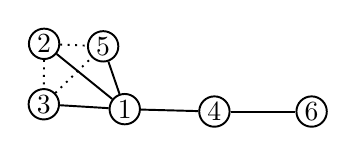
\begin{tikzpicture}
      \node (v1) at (0.5783140174240109, -0.3166613786083942) {$1$};
      \node (v2) at (-0.44575835363976835, 0.5128328399021246) {$2$};
      \node (v3) at (-0.44938111110291284, -0.2545625932461614) {$3$};
      \node (v4) at (1.7169249235942454, -0.3471916538729541) {$4$};
      \node (v5) at (0.3039359827412884, 0.4808427684519154) {$5$};
      \node (v6) at (2.9515342924415832, -0.3471916538729541) {$6$};
      \draw (v1) -- (v2);
      \draw (v1) -- (v3);
      \draw (v1) -- (v4);
      \draw (v1) -- (v5);
      \draw[dotted] (v2) -- (v3);
      \draw[dotted] (v2) -- (v5);
      \draw[dotted] (v3) -- (v5);
      \draw (v4) -- (v6);
      \end{tikzpicture}
    }
  \end{example}
  
\end{frame}

\begin{frame}
\begin{example}<1->[$\Flation{3}{2}{G}$]
    \centering
    \only{
      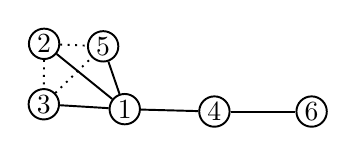
\begin{tikzpicture}
      \node (v1) at (0.5783140174240109, -0.3166613786083942) {$1$};
      \node (v2) at (-0.44575835363976835, 0.5128328399021246) {$2$};
      \node (v3) at (-0.44938111110291284, -0.2545625932461614) {$3$};
      \node (v4) at (1.7169249235942454, -0.3471916538729541) {$4$};
      \node (v5) at (0.3039359827412884, 0.4808427684519154) {$5$};
      \node (v6) at (2.9515342924415832, -0.3471916538729541) {$6$};
      \draw (v1) -- (v2);
      \draw (v1) -- (v3);
      \draw (v1) -- (v4);
      \draw (v1) -- (v5);
      \draw[dotted] (v2) -- (v3);
      \draw[dotted] (v2) -- (v5);
      \draw[dotted] (v3) -- (v5);
      \draw (v4) -- (v6);
      \end{tikzpicture}
    }<1>
    \only{
      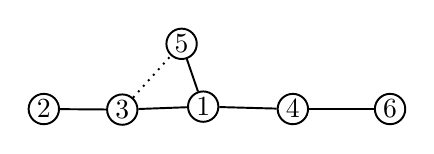
\begin{tikzpicture}
      \node (v1) at (0.5783140174240109, -0.3166613786083942) {$1$};
      \node (v2) at (-1.44575835363976835, -0.3471916538729541) {$2$};
      \node (v3) at (-0.44938111110291284, -0.3545625932461614) {$3$};
      \node (v4) at (1.7169249235942454, -0.3471916538729541) {$4$};
      \node (v5) at (0.3039359827412884, 0.4808427684519154) {$5$};
      \node (v6) at (2.9515342924415832, -0.3471916538729541) {$6$};
      \draw (v1) -- (v3);
      \draw (v1) -- (v4);
      \draw (v1) -- (v5);
      \draw (v2) -- (v3);
      \draw[dotted] (v3) -- (v5);
      \draw (v4) -- (v6);
      \end{tikzpicture}
    }
  \end{example}
\begin{example}<1->[$\Flation{5}{3}{G}$]
    \centering
    \only{
     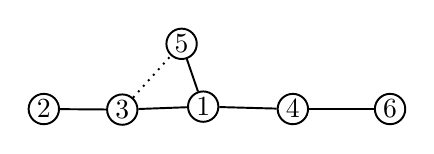
\begin{tikzpicture}
      \node (v1) at (0.5783140174240109, -0.3166613786083942) {$1$};
      \node (v2) at (-1.44575835363976835, -0.3471916538729541) {$2$};
      \node (v3) at (-0.44938111110291284, -0.3545625932461614) {$3$};
      \node (v4) at (1.7169249235942454, -0.3471916538729541) {$4$};
      \node (v5) at (0.3039359827412884, 0.4808427684519154) {$5$};
      \node (v6) at (2.9515342924415832, -0.3471916538729541) {$6$};
      \draw (v1) -- (v3);
      \draw (v1) -- (v4);
      \draw (v1) -- (v5);
      \draw (v2) -- (v3);
      \draw[dotted] (v3) -- (v5);
      \draw (v4) -- (v6);
      \end{tikzpicture}
    }<1>
    \only{
      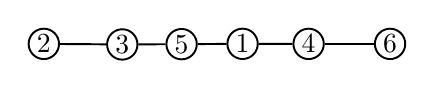
\begin{tikzpicture}
      \node (v1) at (1.0783140174240109, -0.3466613786083942) {$1$};
      \node (v2) at (-1.44575835363976835, -0.3471916538729541) {$2$};
      \node (v3) at (-0.44938111110291284, -0.3545625932461614) {$3$};
      \node (v4) at (1.9169249235942454, -0.3471916538729541) {$4$};
      \node (v5) at (0.3039359827412884, -0.3508427684519154) {$5$};
      \node (v6) at (2.9515342924415832, -0.3471916538729541) {$6$};
      \draw (v1) -- (v4);
      \draw (v1) -- (v5);
      \draw (v2) -- (v3);
      \draw (v3) -- (v5);
      \draw (v4) -- (v6);
      \end{tikzpicture}
    }
  \end{example}
  Ahora para tres $\DynA$-bloques pegados me fijo en un punto de corte y uno dos $\DynA$-bloques en uno y al final me quedan dos $\DynA$ bloques que son de tipo $\DynA_{n}$ y se cumple el lema anterior y esto seria equivalente para $n$-bloques.
\end{frame}


\begin{frame}
	\begin{definitions}
	Una bigráfica cumple la condición de ciclo si todo ciclo tiene un número impar de aristas punteadas.
	\end{definitions}
	\begin{example}<+->
  \centering
  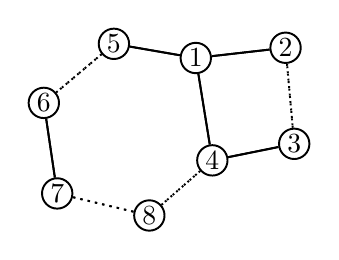
\begin{tikzpicture}
  \node (v0) at (0.89, 1.06) {1};
  \node (v1) at (2.03, 1.19) {2};
  \node (v2) at (2.14, -0.03) {3};
  \node (v3) at (1.1, -0.24) {4};
  \node (v4) at (-0.15, 1.24) {5};
  \node (v5) at (-1.04, 0.49) {6};
  \node (v6) at (-0.87, -0.66) {7};
  \node (v7) at (0.3, -0.94) {8};
  \draw (v0) -- (v1);
  \draw (v0) -- (v3);
  \draw (v0) -- (v4);
  \draw (v1) -- (v0);
  \draw[dotted] (v1) -- (v2);
  \draw[dotted] (v2) -- (v1);
  \draw (v2) -- (v3);
  \draw (v3) -- (v2);
  \draw (v3) -- (v0);
  \draw[dotted] (v3) -- (v7);
  \draw (v4) -- (v0);
  \draw[dotted] (v4) -- (v5);
  \draw[dotted] (v5) -- (v4);
  \draw (v5) -- (v6);
  \draw (v6) -- (v5);
  \draw[dotted] (v6) -- (v7);
  \draw[dotted] (v7) -- (v6);
  \draw[dotted] (v7) -- (v3);
\end{tikzpicture}
  \end{example}
\end{frame}

\begin{frame}{$\DynD$-nucleo}
  \begin{itemize}
  \item Una bigráfica cíclica $ H = x_{1} - x_{2} - \cdots - x_{h}-x_{1}$ (todos los $x_{i}$ distintos para $ 1 \leq i \leq h$) que satisface la condición de ciclo.
  \item A esta bigráfica $H$ le llamaremos el $\DynD$-núcleo.
  \end{itemize}
\end{frame}

\section{Descripción de el problema}
\begin{frame}{Descripción de el problema}
  \begin{itemize}
     \item El problema propuesto es la clasificación algorítmica en gráficas de tipo $\DynD_{n}$
     \item Para esto se propone usar el algoritmo de componentes triconexas para caracterizar las de tipo $\DynD_{n}$
    \end{itemize}	
\end{frame}

\section{Componentes triconexas}
\begin{frame}{Algoritmo de Componentes triconexas}
  \begin{enumerate}
  	\item Divide las aristas múltiples para formar enlaces triples y un grafo biconexo simple $G'$.
    \item Encuentra los componentes de separación de $G'$.
    \item Combina los enlaces triples y triángulos en enlaces y polígonos.
  \end{enumerate}
\end{frame}

\begin{frame}{Componentes triconexas}
Sea $G = (V, E)$ un multigráfo y sea $H = (W, F)$ un subgráfo de $G$, definimos una relación de equivalencia sobre $E - F$ como sigue:
  \begin{definitions}
    \begin{enumerate}
    \item $\forall e \in E - F$, $e \widetilde{=} e$.
    \item $\forall e, f \in E - F$, $e \widetilde{=} f$ si y solo si existe un camino que une $e, f$ que no tiene un vértice en $W$.
    \end{enumerate}
  \end{definitions}
\end{frame}

\begin{frame}{Componentes triconexas}
Si $H = \{\{a, b\}, \emptyset\}$, las clases de equivalencia son llamadas clases de separación relativas al par $\{a, b\}$.
  \begin{definitions}
    \begin{itemize}
      \item Sean $S_1,S_2,\ldots, S_k$, las clases de separación relativas al par $(a,b)$. Si existe una partición $(A,B)$ de $\{1,2, . . . , k\}$ tal que $|E_{1} = \bigcup_{i \in A} S_i| \geq 2$ y $ |E_{2}= \bigcup_{j \in B} S_j| \geq 2$, decimos que $\{a,b\}$ es un par de separación.
    \end{itemize}
  \end{definitions}
\end{frame}

\begin{frame}{Componentes triconexas}
  \begin{definitions}
    \begin{itemize}
     \item Si $G$ es biconexa y $G$ no tiene par de separación entonces $G$ es triconexa.
     \end{itemize}
  \end{definitions}
  \centering
  \begin{example}<+->
  \quad
  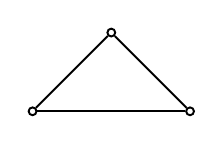
\begin{tikzpicture}[baseline=(current bounding box.center)]
  \node (v0) at (1, 0) {};
  \node (v1) at (-1, 0) {};
  \node (v2) at (0.0, 1) {};
  \draw (v0) -- (v1);
  \draw (v0) -- (v2);
  \draw (v2) -- (v1);
  \end{tikzpicture}
  \quad
  \quad
  \quad
  \quad
  \quad
  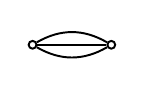
\begin{tikzpicture}
	\node(v0) at (0,0) {};
	\node(v1) at (1,0) {};
	\draw (v0) to (v1);
	\draw (v0) to[bend right] (v1);
	\draw (v1) to[bend right] (v0);
  \end{tikzpicture}
  \quad
  \quad
  \quad
  \quad
  \quad
  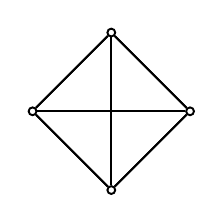
\begin{tikzpicture}[baseline=(current bounding box.center)]
  \node (v0) at (1, 0.) {};
  \node (v1) at (-1, 0) {};
  \node (v2) at (0.0, -1) {};
  \node (v3) at (0.0, 1) {};
  \draw (v0) -- (v1);
  \draw (v0) -- (v2);
  \draw (v0) -- (v3);
  \draw (v1) -- (v0);
  \draw (v1) -- (v2);
  \draw (v1) -- (v3);
  \draw (v2) -- (v1);
  \draw (v2) -- (v0);
  \draw (v2) -- (v3);
  \draw (v3) -- (v2);
  \draw (v3) -- (v1);
  \draw (v3) -- (v0);
  \end{tikzpicture}
  \quad
  \end{example}
\end{frame}

\begin{frame}{La operación de división}
  Sea $G$ el bigrafo y $H=\{\{2, 3\},  \emptyset\}$
\begin{example}<+->
  \centering
  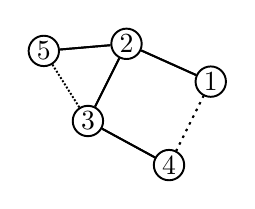
\begin{tikzpicture}
  \node (v0) at (1.15, 0.21) {1};
  \node (v1) at (0.08, 0.69) {2};
  \node (v2) at (-0.41, -0.29) {3};
  \node (v3) at (0.62, -0.85) {4};
  \node (v4) at (-0.97, 0.6) {5};
  \draw (v0) -- (v1);
  \draw[dotted] (v0) -- (v3);
  \draw (v1) -- (v0);
  \draw (v1) -- (v4);
  \draw (v1) -- (v2);
  \draw[dotted] (v2) -- (v4);
  \draw (v2) -- (v3);
  \draw (v2) -- (v1);
  \draw (v3) -- (v2);
  \draw[dotted] (v3) -- (v0);
  \draw (v4) -- (v1);
  \draw[dotted] (v4) -- (v2);
  \end{tikzpicture}
  \end{example}
  \begin{block}{}
 La clase de equivalencia de $2\rule[1mm]{4mm}{0.3mm}5$ es el conjunto:\\
$S_{1} = \{2\rule[1mm]{4mm}{0.3mm}5, 5 \hdashrule[1mm]{4mm}{1pt}{1pt} 3\}$\\
La clase de equivalencia de $1\hdashrule[1mm]{4mm}{1pt}{1pt} 4$ es el conjunto:\\
$S_{2} = \{2 \hdashrule[1mm]{4mm}{1pt}{1pt} 1, 1\rule[1mm]{4mm}{0.3mm}4, 4\rule[1mm]{4mm}{0.3mm}3\}$\\
La clase de equivalencia de $2\rule[1mm]{4mm}{0.3mm}3$ es el conjunto:\\
$S_{3} = \{2\rule[1mm]{4mm}{0.3mm}3\}$\\ 
  \end{block}
\end{frame}

\begin{frame}{La operación de división}
\begin{block}{}
Para saber si $\{2,3\}$ es un par de separación hay que encontrar una partición de $\{1, 2, 3\} = A \cup B$, $A \cap B = \{\emptyset\}$ tal que se cumple que $|E_{1} = \bigcup_{i \in A} S_i| \geq 2$ y $ |E_{2}= \bigcup_{j \in B} S_j| \geq 2$.\\
\end{block}
\begin{block}{}
 En este caso $A = \{1, 3\}$, $B=\{2\}$ es una partición posible que buscamos y entonces  $\{2, 3\}$ es un par de separación.\\
\end{block}
\end{frame}

\begin{frame}{La operación de división}
\begin{block}{}
Ahora supongamos $\{a, b\}$ es un par de separación. \\Si $H=\{\{a, b\}, \emptyset\}$ y $S_{1},S_{2}, \ldots, S_{k}$ son las clases de separación del par $\{a, b\}$(las clases de equivalencia definidas por $H$).
\end{block}
\begin{block}{}
Sea $A, B$ la partición del conjunto $\{1,2,\ldots,k\}$ tal que $|E_1 = \bigcup_{i \in A} S_i| \geq 2$ y $ |E_{2}= \bigcup_{j \in B} S_j| \geq 2$. 
\end{block}
\end{frame}

\begin{frame}
\begin{block}{}
Si $H_{1} = (V(E_{1}), E_{1})$ y $H_{2} = (V(E_{2}), E_{2})$ entonces, $V(E_{1}) \cap V(E_{1}) = \{a, b\}$ donde la arista $a\rule[1mm]{4mm}{0.3mm} b$ es llamada arista virtual.
\end{block}
\begin{block}{}
Sea $G_{i} = H_{i} + a\rule[1mm]{4mm}{0.3mm} b$ para $i \in \{1, 2\}$.\\ Las $G_{i}$ son los bigrafos de división de $G$ en $\{a, b\}$. 
\end{block}
\end{frame}

\begin{frame}
Donde $A=\{1,3\}$ y $B=\{2\}$ 
\begin{example}<+->
  \quad
  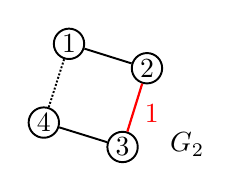
\begin{tikzpicture}
  \node (v0) at (-0.5, 0.78) {1};
  \node (v1) at (0.49, 0.47) {2};
  \node (v2) at (0.18, -0.53) {3};
  \node (v3) at (-0.82, -0.22) {4};
  \draw[dotted] (v0) -- (v3);
  \draw (v0) -- (v1);
  \draw [thick, red] (v1) -- (v2) ;
  \node[draw = none, shape = rectangle, fill=none, red] at (0.55, -0.1) {$1$};  
  \draw (v2) -- (v3);
  \draw[dotted] (v3) -- (v0);
  \node[draw = none, shape = rectangle, fill=none] at (1, -0.5) {$G_{2}$};
  \end{tikzpicture}
  \quad
  \quad
  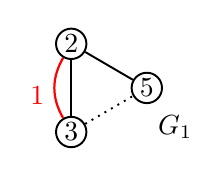
\begin{tikzpicture}
  \node (v0) at (0.64, 0.0) {5};
  \node (v1) at (-0.32, -0.56) {3};
  \node (v2) at (-0.32, 0.56) {2};
  \draw (v0) -- (v2);
  \draw (v1) -- (v2);
  \draw[dotted] (v1) -- (v0);
  \draw[thick, red] (v2) to[bend right] (v1);
  \node[draw = none, shape = rectangle, fill=none, red] at (-0.75, -0.1) {$1$};
  \node[draw = none, shape = rectangle, fill=none] at (1, -0.5) {$G_{1}$};
  \end{tikzpicture}
  \end{example}
\end{frame}

\begin{frame}{La operación de división}
\begin{example}<+->
  \quad
  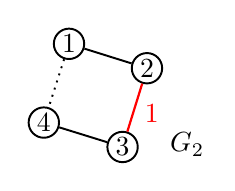
\begin{tikzpicture}
  \node (v0) at (-0.5, 0.78) {1};
  \node (v1) at (0.49, 0.47) {2};
  \node (v2) at (0.18, -0.53) {3};
  \node (v3) at (-0.82, -0.22) {4};
  \draw[dotted] (v0) -- (v3);
  \draw (v0) -- (v1);
  \draw [thick, red] (v1) -- (v2) ;
  \node[draw = none, shape = rectangle, fill=none, red] at (0.55, -0.1) {$1$}; 
  \draw (v2) -- (v3);
  \node[draw = none, shape = rectangle, fill=none] at (1, -0.5) {$G_{2}$};
  \end{tikzpicture}
  \quad
  \quad
  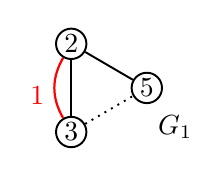
\begin{tikzpicture}
  \node (v0) at (0.64, 0.0) {5};
  \node (v1) at (-0.32, -0.56) {3};
  \node (v2) at (-0.32, 0.56) {2};
  \draw (v0) -- (v2);
  \draw (v1) -- (v2);
  \draw[dotted] (v1) -- (v0);
  \draw[thick, red] (v2) to[bend right] (v1);
  \node[draw = none, shape = rectangle, fill=none, red] at (-0.75, -0.1) {$1$};
  \node[draw = none, shape = rectangle, fill=none] at (1, -0.5) {$G_{1}$};
  \end{tikzpicture}
  \end{example}
  \begin{itemize}
	\item Como $G_{1}$ y $G_{2}$ no son triconexas(tiene pares de separación) entonces, supongamos que sabemos que $\{1, 3\}$ es un par de separación de $G_{2}$ y el mismo par $\{2, 3\}$ es un par de separación de $G_{1}$ entonces,
	\end{itemize}
\end{frame}

\begin{frame}{La operación de división}
\begin{itemize}
  \begin{example}<+->
  \quad
  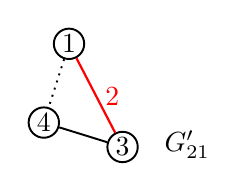
\begin{tikzpicture}
  \node (v0) at (-0.5, 0.78) {1};
  \node (v2) at (0.18, -0.53) {3};
  \node (v3) at (-0.82, -0.22) {4};
  \draw[dotted] (v0) -- (v3);
  \draw (v2) -- (v3);
  \draw [thick, red] (v0) -- (v2) ;
  \node[draw = none, shape = rectangle, fill=none, red] at (0.05, 0.11) {$2$};
  \node[draw = none, shape = rectangle, fill=none] at (1, -0.5) {$G'_{21}$};
  \end{tikzpicture}
  \quad
  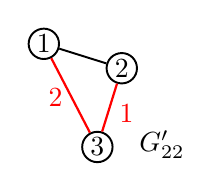
\begin{tikzpicture}
  \node (v0) at (-0.5, 0.78) {1};
  \node (v1) at (0.49, 0.47) {2};
  \node (v2) at (0.18, -0.53) {3};
  \draw (v0) -- (v1);
  \draw [thick, red] (v0) -- (v2) ;
  \node[draw = none, shape = rectangle, fill=none, red] at (-0.35, 0.1) {$2$};
  \draw [thick, red] (v1) -- (v2) ;
  \node[draw = none, shape = rectangle, fill=none, red] at (0.55, -0.1) {$1$};
  \node[draw = none, shape = rectangle, fill=none] at (1, -0.5) {$G'_{22}$};
  \end{tikzpicture}
  \quad
  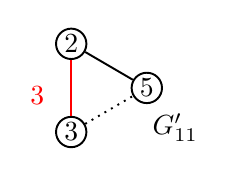
\begin{tikzpicture}
  \node (v0) at (0.64, 0.0) {5};
  \node (v1) at (-0.32, -0.56) {3};
  \node (v2) at (-0.32, 0.56) {2};
  \draw (v0) -- (v2);
  \draw[thick, red] (v1) -- (v2);
  \draw[dotted] (v1) -- (v0);
  \node[draw = none, shape = rectangle, fill=none, red] at (-0.75, -0.1) {$3$};
  \node[draw = none, shape = rectangle, fill=none] at (1, -0.5) {$G'_{11}$};
  \end{tikzpicture}
  \quad
  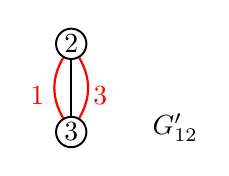
\begin{tikzpicture}
  \node (v1) at (-0.32, -0.56) {3};
  \node (v2) at (-0.32, 0.56) {2};
  \draw (v1) -- (v2);
  \draw[thick, red] (v2) to[bend right] (v1);
  \draw[thick, red] (v2) to[bend left] (v1);
  \node[draw = none, shape = rectangle, fill=none, red] at (-0.75, -0.1) {$1$};
  \node[draw = none, shape = rectangle, fill=none, red] at (0.05, -0.1) {$3$};
  \node[draw = none, shape = rectangle, fill=none] at (1, -0.5) {$G'_{12}$};
  \end{tikzpicture}
  \end{example}
  \item Ahora tenemos componentes triconexos. Estos son llamados componentes de división.\\
 \end{itemize}
\end{frame}

\begin{frame}{La operación de división}
  El siguiente resultado es debido a Hopcroft and Tarjan.
  \begin{lemma}
   El número total de aristas en todos los componentes de división no excede $3|E| - 6$
  \end{lemma}
\end{frame}

\begin{frame}{La operación de unión}
	\begin{itemize}
	\item Sean $H_{1}$ y $H_{2}$ componentes de división de $G$ tal que ambas contengan la misma arista virtual 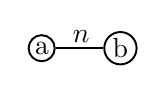
\begin{tikzpicture}
	\node(v0) at (0,0) {a};
	\node(v1) at (1,0) {b};
	\draw (v0) to (v1);
	\node[draw = none, shape = rectangle, fill=none] at (0.5, 0.15) {$n$};
  \end{tikzpicture}
	\item Combinamos estos dejando que $H = H_{1} + H_{2} - (a, b, n)$. 
	\end{itemize}
\end{frame}

\begin{frame}{La operación de unión}
	Pero solo vamos a fusionar  los componentes de división de la siguiente forma:
	\begin{enumerate}
		\item Fusionamos 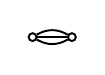
\begin{tikzpicture}
	\node(v0) at (0,0) {};
	\node(v1) at (.5,0) {};
	\draw (v0) to (v1);
	\draw (v0) to[bend right] (v1);
	\draw (v1) to[bend right] (v0);
  \end{tikzpicture} tanto como sea posible
	 	\item Fusionamos \begin{tikzpicture}
  \node (v0) at (0.5, 0) {};
  \node (v1) at (-.5, 0) {};
  \node (v2) at (0.0, -.5) {};
  \draw (v0) -- (v1);
  \draw (v0) -- (v2);
  \draw (v2) -- (v1);
  			\end{tikzpicture} tanto como sea posible.
		\end{enumerate}
	 El conjunto final de grafos es llamado conjunto completo de componentes de triconexas.
\end{frame}

\begin{frame}{}
  \begin{lemma}
   Un conjunto completo de componentes triconexas es único hasta isomorfismo.
  \end{lemma}
\end{frame}

\section{Planteamiento de el problema}
\begin{frame}{}
	\begin{itemize}
	\item La conjetura es que la clasificación quedara como las componentes triconexas completas son bloques de tipo $A_{n}$.
	\item Me tomo un grafo le quito sus componentes biconexas y compruebo que todas excepto una componente son $\DynA$-bloques ahora para comprobar que la componente biconexa que no es $\DynA$-bloque es de tipo $\DynD_{n}$ utilizo el algoritmo de descomposición en componentes triconexas.
	\end{itemize}
\end{frame}

\begin{frame}{}
	\begin{itemize}
	\item Del conjunto de componentes triconexas nos interesa recuperar los componentes biconexas, por ejemplo de $G'_{21}, G'_{22}$ obtenemos la subgráfica inducida, \begin{tikzpicture}
  \node (v0) at (-0.5, 0.78) {1};
  \node (v1) at (0.49, 0.47) {2};
  \node (v2) at (0.18, -0.53) {3};
  \node (v3) at (-0.82, -0.22) {4};
  \draw[dotted] (v0) -- (v3);
  \draw (v0) -- (v1);
  \draw (v1) -- (v2) ;
  \draw (v2) -- (v3);
  \end{tikzpicture}  y de $G'_{11}$ y $G'_{12}$ es otra subgráfica inducida \begin{tikzpicture}
  \node (v0) at (0.64, 0.0) {5};
  \node (v1) at (-0.32, -0.56) {3};
  \node (v2) at (-0.32, 0.56) {2};
  \draw (v0) -- (v2);
  \draw (v1) -- (v2);
  \draw[dotted] (v1) -- (v0);
  \end{tikzpicture}
  \item en este caso el conjunto completo de componentes biconexas.
  \item De este ejemplo tenemos que una subgráfica cumple la condición de ciclo y una que es un $\DynA$-bloque. por lo tanto $G$ es de tipo $\DynD_{5}$.
	\end{itemize}
\end{frame}

\appendix

\section*{Apéndice}

\subsection*{Bibiográfia}
\begin{frame}[allowframebreaks]{Bibiográfia}

\beamertemplatebookbibitems
\begin{thebibliography}{1}
%\bibitem{Autor1990}A. Autor. \newblock\emph{Manual de Lo que sea}.\newblock
%Editorial, 1990.\beamertemplatearticlebibitems

\bibitem{Abarca2016}M. Abarca \& D. Rivera\newblock Graph Theoretical and 
Algorithmic Characterizations of Positive Definite Symmetric Quasi-Cartan 
Matrices\emph{.}
\newblock\emph{Fundamenta Informaticae}. 149(3):241--261, 2016.

\bibitem{Kiem-Phong Vo1983}Kiem-Phong Vo \newblock Finding triconnected components of graphs\emph{.}
\newblock\emph{Linear and Multilinear Algebra.} 13:2, 143-165, 1983

\bibitem{Abarca2011}M. Abarca.\newblock Algoritmo Para Decidir si una
Forma Unitaria es de Tipo $\DynA_{n}$(Tesis de Licenciatura)\emph{.} 2011

\end{thebibliography}
\end{frame}
\end{document}